% Pandoc template for paper/main.tex (used by scripts/export_paper.mjs via --template).
% Written for pdfLaTeX (arXiv's default); it also compiles with XeTeX/Tectonic.
\documentclass[11pt,a4paper]{article}
\usepackage[T1]{fontenc}
\usepackage[utf8]{inputenc}
\usepackage{lmodern}
\usepackage{textcomp}
\usepackage{microtype}
\usepackage[margin=25mm]{geometry}
\usepackage{amsmath,amssymb}
\usepackage{graphicx}
\usepackage{booktabs,longtable,array,calc,multirow}
\usepackage{etoolbox}
\usepackage[labelformat=empty,font=small,skip=6pt]{caption}
\usepackage{newunicodechar}
\usepackage[hidelinks]{hyperref}
\hypersetup{pdftitle={Flight-testing a fruit-fly connectome as an aircraft yaw damper}, pdfauthor={Mutaqin Aryawijaya}}
\usepackage{url}

% The caption text already starts with "Figure N." / "Table N.", as in the web paper.
\AtBeginEnvironment{longtable}{\small\setlength{\tabcolsep}{4pt}}
\setlength{\LTpre}{\medskipamount}\setlength{\LTpost}{\medskipamount}
\setcounter{secnumdepth}{-1}   % section numbers are part of the heading text
\setlength{\parindent}{1.4em}
\providecommand{\tightlist}{\setlength{\itemsep}{0pt}\setlength{\parskip}{0pt}}
\makeatletter
\newsavebox\pandoc@box
\newcommand*\pandocbounded[1]{\sbox\pandoc@box{#1}%
  \Gscale@div\@tempa{\textheight}{\dimexpr\ht\pandoc@box+\dp\pandoc@box\relax}%
  \Gscale@div\@tempb{\linewidth}{\wd\pandoc@box}%
  \ifdim\@tempb\p@<\@tempa\p@\let\@tempa\@tempb\fi
  \ifdim\@tempa\p@<\p@\scalebox{\@tempa}{\usebox\pandoc@box}\else\usebox{\pandoc@box}\fi}
\makeatother
\renewcommand{\topfraction}{.9}\renewcommand{\textfraction}{.08}\renewcommand{\floatpagefraction}{.8}
\urlstyle{same}
\setlength{\emergencystretch}{3em}   % long runs of non-breaking spaces in the web text

% Unicode characters that the web paper uses in running text
\newunicodechar{−}{\ensuremath{-}}
\newunicodechar{×}{\ensuremath{\times}}
\newunicodechar{±}{\ensuremath{\pm}}
\newunicodechar{≤}{\ensuremath{\leq}}
\newunicodechar{≥}{\ensuremath{\geq}}
\newunicodechar{≈}{\ensuremath{\approx}}
\newunicodechar{∈}{\ensuremath{\in}}
\newunicodechar{→}{\ensuremath{\rightarrow}}
\newunicodechar{↓}{\ensuremath{\downarrow}}
\newunicodechar{∞}{\ensuremath{\infty}}
\newunicodechar{√}{\ensuremath{\surd}}
\newunicodechar{∑}{\ensuremath{\sum}}
\newunicodechar{∫}{\ensuremath{\int}}
\newunicodechar{ℓ}{\ensuremath{\ell}}
\newunicodechar{°}{\ensuremath{^\circ}}
\newunicodechar{π}{\ensuremath{\pi}}
\newunicodechar{α}{\ensuremath{\alpha}}
\newunicodechar{β}{\ensuremath{\beta}}
\newunicodechar{γ}{\ensuremath{\gamma}}
\newunicodechar{δ}{\ensuremath{\delta}}
\newunicodechar{ε}{\ensuremath{\varepsilon}}
\newunicodechar{λ}{\ensuremath{\lambda}}
\newunicodechar{μ}{\ensuremath{\mu}}
\newunicodechar{σ}{\ensuremath{\sigma}}
\newunicodechar{τ}{\ensuremath{\tau}}
\newunicodechar{ω}{\ensuremath{\omega}}
\newunicodechar{Δ}{\ensuremath{\Delta}}
\newunicodechar{𝒮}{\ensuremath{\mathcal{S}}}
\newunicodechar{𝒯}{\ensuremath{\mathcal{T}}}
\newunicodechar{𝒱}{\ensuremath{\mathcal{V}}}
\newunicodechar{ν}{\ensuremath{\nu}}
\newunicodechar{ζ}{\ensuremath{\zeta}}
\newunicodechar{φ}{\ensuremath{\phi}}
\newunicodechar{§}{\S{}}
\newunicodechar{Σ}{\ensuremath{\Sigma}}
\newunicodechar{ }{~}
\newunicodechar{ }{\,}
\newunicodechar{ }{\,}
\newunicodechar{ }{\enspace}
\newunicodechar{ }{\quad}
\newunicodechar{‑}{-}

\title{Flight-testing a fruit-fly connectome as an aircraft yaw damper}
\author{Mutaqin
Aryawijaya\\[2pt] \normalsize Independent researcher\\[1pt] \small \href{mailto:mutaqin@aryawijaya.com}{mutaqin@aryawijaya.com}\\[1pt] \small ORCID: \href{https://orcid.org/0009-0008-5199-2413}{0009-0008-5199-2413}\\[2pt] \small Code and data: \url{https://github.com/aryawidjaja/flight-test-the-fly}}
\date{October 2026}

\begin{document}
\maketitle
\begin{abstract}
\noindent Flight-control laws are assessed by their frequency response,
stability margins, gust rejection and behaviour under failure;
connectome-derived controllers have so far been shown mainly in
time-domain demonstrations. We applied these tests to a spiking model of
the fruit fly's visual yaw pathway, a 20,556-neuron FlyWire subcircuit
from the T4/T5 motion detectors to the descending neuron DNa02, with the
aircraft's yaw rate imposed directly as the firing rate of artificial
T4/T5 sources, and compared it with rewired copies and a classical yaw
damper. Under sinusoidal yaw, the right-minus-left DNa02 firing rate
followed the yaw rate with coherence 0.98 at 1~Hz and with the
stabilizing sign. It ranked first against 19 degree-preserving rewirings
(median 0.31; \emph{p}~=~0.05) and narrowly first against 19
cell-type-preserving rewirings, which leave every input to the HS, VS,
H2 and DNa02 cells unchanged. Closed around the rudder of a simulated
six-degree-of-freedom Cessna 172 in moderate turbulence and tuned under
the same margin rule as the yaw damper, it reduced RMS yaw rate by 19\%,
against 57\% for the damper. Of 11 wirings it had the lowest RMS yaw
rate and the lowest RMS sideslip on both aircraft models. The three
rewired controllers that came closest on yaw rate in the Cessna model
were saturated relays flying skidding turns. No lesion-study flight
departed, so the pre-specified departure test could not separate the
wirings; under random neuron loss the real wiring's mean RMS yaw rate
rose toward the bare airframe's but not above it, partly because the
loss often silenced its one active readout neuron, and silencing its six
HS cells returned it to the bare airframe's yaw rate. Flight-control
tests can therefore measure what a connectome's wiring contributes to a
controller, and they expose failure modes, such as relay-like skidding,
that a single performance score hides.
\end{abstract}

\protect\phantomsection\label{s1}
\section{\texorpdfstring{1\quad Introduction}{1Introduction}}\label{introduction}

\noindent A complete synaptic wiring diagram of an adult fruit-fly brain
is now public \cite{dorkenwald2024,schlegel2024}, and a leaky
integrate-and-fire network run directly on an earlier release of that
diagram (v630), with one free parameter, reproduces a range of measured
sensorimotor responses \cite{shiu2024}. A model of this kind can be
placed in a feedback loop with a machine. That raises an engineering
question that is easy to state and has rarely been tested with
engineering tools: how a piece of real wiring behaves as a controller.

Aeronautics has a standard way of answering this question for a new
flight-control law. Its frequency response is measured, its gain and
phase margins are checked against minimum values \cite{milf94901975},
its rejection of gusts is evaluated in standard turbulence models
\cite{milf87851980}, and its behaviour is examined as its components
fail. We applied this procedure to the yaw axis, which needs a short
vocabulary. The \emph{yaw rate} \emph{r} is how fast the nose swings
left or right. \emph{Sideslip} \emph{β} is the angle between the nose
and the oncoming air; a plane that turns with its rudder held over
``skids'' with large sideslip. Gusts excite the \emph{Dutch roll}, a
lightly damped oscillation in which yaw and sideslip trade back and
forth. A \emph{yaw damper} is the classical autopilot that measures
\emph{r} and moves the rudder to oppose it.

The fly's own yaw stabilization offers a natural test case. When a fly
turns, the image of the world slides across both eyes.
Direction-selective T4 and T5 neurons in the optic lobe signal this
motion, and their a and b subtypes prefer front-to-back and
back-to-front motion, respectively \cite{maisak2013,shinomiya2019}.
Horizontal-system (HS) tangential cells are excited by front-to-back
motion on their own side \cite{schnell2010}, and activating HS cells on
one side turns the fly toward that side \cite{haikala2013}. Among the
descending neurons that carry commands to the body \cite{namiki2018},
the right-minus-left difference in DNa02 activity predicts turning
velocity in walking flies \cite{rayshubskiy2025}. Chained together,
these facts predict an optomotor reflex that opposes an imposed
rotation. In tethered flight this response has delays of tens of
milliseconds \cite{theobald2010}.

Several recent projects place connectome models in a flight loop,
usually with time-domain demonstrations and sometimes with
shuffled-wiring controls \cite{clutch2026,leohio2026,flygm2026};
shuffled controls are also standard in the connectome-modelling
literature \cite{shiu2024}. Descending-neuron dynamics have been
measured in real insects \cite{leibbrandt2021}, and the fly's yaw
optomotor response has been identified behaviourally
\cite{theobald2010}. We could not find prior work that measures the
frequency response of a connectome-model controller, its gain and phase
margins by breaking the loop, its behaviour in standard Dryden
turbulence \cite{milf87851980}, or curves of its degradation under
graded neuron loss toward departure, nor work that compares a connectome
rudder loop with a classical yaw damper under an identical tuning
budget.

We tested four hypotheses, fixed before any brain or flight simulation:
that the circuit tracks yaw rotation coherently and with the stabilizing
sign, and better than rewired copies (H1); that, closed around a rudder,
it lowers RMS yaw rate against the bare airframe and beats the median
rewired copy given the same tuning, on a two-state model (H2) and on a
six-degree-of-freedom simulator (H3); and that it degrades more
gracefully than rewired copies as neurons are silenced (H4). The goal
was not to beat the yaw damper, but to measure how a controller taken
from a connectome behaves and whether its real wiring matters. H1, H2
and H3 were supported: the real wiring encoded yaw rate with the
stabilizing sign and, in closed loop, damped yaw motion more than any of
the ten rewired copies tested (rank 1 of 11, \emph{p}~=~0.091) but far
less than the classical yaw damper. H4 could not be tested, because no
flight departed.

\protect\phantomsection\label{s2}
\section{\texorpdfstring{2\quad Methods}{2Methods}}\label{methods}

\subsection{\texorpdfstring{2.1\quad Connectome
subcircuit}{2.1Connectome subcircuit}}\label{connectome-subcircuit}

\noindent We used the FlyWire connectome, materialization v783
\cite{dorkenwald2024}, with its cell-type annotations
\cite{schlegel2024} and the signed connectivity table distributed with
the whole-brain model of Shiu et al. \cite{shiu2024}. Keeping only
connections of at least 5 synapses, we took as sources 𝒮 all T4a--d and
T5a--d cells and as targets 𝒯 the descending neurons DNa02 and
DNg02\textsubscript{a--h}, and kept every neuron that lies on a directed
path of at most 4 hops from a source to a target,

\[\mathcal{V}=\bigl\{\,i:\ d(\mathcal{S}\!\to\! i)+d(i\!\to\!\mathcal{T})\le 4\,\bigr\}\tag{1}\]

\noindent where \emph{d} is the shortest directed hop count, together
with every connection of at least 5 synapses among those neurons,
recurrent ones included. The subcircuit holds 20,556 neurons: 12,056
T4/T5 cells and 8,500 others, among them 6 HS, 16 VS and 2 H2 cells, 2
DNa02 cells (one per side) and 22 DNg02 cells. It has 283,576
connections, of which 251,358 are simulated; the 32,218 connections onto
T4/T5 cells are dropped because those cells are replaced by input
sources (Section 2.3). T4/T5 cells supply 83\% of all synapses onto HS
cells, and 99.97\% of that input comes from the front-to-back a
subtypes.

\subsection{\texorpdfstring{2.2\quad Neuron
model}{2.2Neuron model}}\label{neuron-model}

\noindent All non-input neurons follow the leaky integrate-and-fire
model of Shiu et al. \cite{shiu2024}, unchanged. Each neuron \emph{i}
has a membrane potential \emph{v}\textsubscript{\emph{i}} and a synaptic
variable \emph{g}\textsubscript{\emph{i}},

\[\tau_m\frac{dv_i}{dt}=v_0-v_i+g_i,\qquad \tau_s\frac{dg_i}{dt}=-g_i,\tag{2}\]

\noindent and a spike of presynaptic neuron \emph{j} arrives after a
fixed delay,

\[\begin{gathered}g_i\leftarrow g_i+w_{\mathrm{syn}}\,W_{ji}\ \ \text{at}\ \ t_j^{\mathrm{spk}}+t_{\mathrm{dly}},\\ v_i>v_{\mathrm{th}}\ \Rightarrow\ v_i\leftarrow v_{\mathrm{reset}},\ \ g_i\leftarrow 0,\end{gathered}\tag{3}\]

\noindent where \emph{W\textsubscript{ji}} is the synapse count from
\emph{j} to \emph{i}, signed by the presynaptic neurotransmitter
(GABAergic and glutamatergic neurons inhibitory, others excitatory).
After a spike, \emph{v} and \emph{g} stop evolving for
\emph{t}\textsubscript{ref} (\emph{g} still receives synaptic input).
Parameters are listed in Table~1. The network was simulated in Brian~2
with exact integration of the linear dynamics.

\protect\phantomsection\label{t-params}
\begin{longtable}[]{@{}lr@{}}
\caption{\textbf{Table 1. Model and controller parameters.} The neuron
parameters are those of the published whole-brain model; the input and
readout parameters were fixed before any brain or flight simulation,
except the washout, which was fixed after the pilot runs (Section
2.9).}\tabularnewline
\toprule\noalign{}
Parameter & Value \\
\midrule\noalign{}
\endfirsthead
\toprule\noalign{}
Parameter & Value \\
\midrule\noalign{}
\endhead
\bottomrule\noalign{}
\endlastfoot
Resting and reset potential, \emph{v}\textsubscript{0},
\emph{v}\textsubscript{reset} & −52, −52 mV \\
Threshold, \emph{v}\textsubscript{th} & −45 mV \\
Membrane time constant, \emph{τ}\textsubscript{m} & 20 ms \\
Synaptic time constant, \emph{τ}\textsubscript{s} & 5 ms \\
Refractory period, \emph{t}\textsubscript{ref} & 2.2 ms \\
Synaptic delay, \emph{t}\textsubscript{dly} & 1.8 ms \\
Weight per synapse, \emph{w}\textsubscript{syn} & 0.275 mV \\
Integration step, Δ\emph{t} & 0.1 ms \\
T4/T5 baseline rate, \emph{r}\textsubscript{base} & 10 Hz \\
Input gain, \emph{γ} & 1 Hz per °/s \\
Control step, \emph{T}\textsubscript{c} & 10 ms \\
Washout time constant, \emph{τ}\textsubscript{w} (fly and damper) & 1
s \\
\end{longtable}

\subsection{\texorpdfstring{2.3\quad Visual input
encoding}{2.3Visual input encoding}}\label{visual-input-encoding}

\noindent We take \emph{r}~\textgreater~0 as a nose-right rotation. A
nose-right turn moves the visual world front-to-back across the left eye
and back-to-front across the right eye; T4a/T5a prefer front-to-back and
T4b/T5b back-to-front motion \cite{maisak2013,shinomiya2019}. Each T4/T5
cell \emph{c} was therefore replaced by an independent Poisson source
with rate

\[\lambda_c(t)=r_{\mathrm{base}}+\gamma\,\max\bigl(0,\ s_c\,r(t)\bigr),\tag{4}\]

\noindent with \emph{r} in degrees per second,
\emph{s\textsubscript{c}}~=~+1 for left T4a/T5a and right T4b/T5b cells,
\emph{s\textsubscript{c}}~=~−1 for left T4b/T5b and right T4a/T5a cells,
and \emph{s\textsubscript{c}}~=~0 for the vertical-motion c and d
subtypes. In each integration step Δ\emph{t} a source fires with
probability \emph{λ\textsubscript{c}}Δ\emph{t}. This encoding is
piecewise linear (half-wave rectified) in \emph{r} for each cell and
ignores the temporal-frequency tuning of real motion detectors (Section
4.5).

\subsection{\texorpdfstring{2.4\quad Readout and
controllers}{2.4Readout and controllers}}\label{readout-and-controllers}

\noindent The controller output is the rudder command
\emph{u}~∈~{[}−1,~1{]}, with \emph{u}~\textgreater~0 commanding a
nose-right moment and \textbar{}\emph{u}\textbar~=~1 equal to 16° of
rudder. The brain and the aircraft advance in lockstep with control step
\emph{T}\textsubscript{c}. In closed loop the T4/T5 sources are driven
by the sampled yaw rate, \emph{r}(\emph{t})~=~\emph{r\textsubscript{k}}
for
\emph{t}~∈~{[}\emph{kT}\textsubscript{c},~(\emph{k}~+~1)\emph{T}\textsubscript{c})
(sample-and-hold). Let
Δ\textsubscript{\emph{k}}~=~\emph{ν}\textsubscript{R,\emph{k}}~−~\emph{ν}\textsubscript{L,\emph{k}}
be the right-minus-left DNa02 firing rate (Hz) over that window, driven
by \emph{r\textsubscript{k}}, and \emph{b} its mean over a 1~s warm-up
without rotation before each flight. The fly controller is

\[\begin{gathered}x_k=\Delta_{k-1}-b,\qquad a=e^{-T_c/\tau_w},\\ \ell_k=a\,\ell_{k-1}+(1-a)\,x_k,\\ u_k=\operatorname{sat}\bigl(\varepsilon K\,(x_k-\ell_k)\bigr),\end{gathered}\tag{5}\]

\noindent with ℓ\textsubscript{0}~=~0 and \emph{u}\textsubscript{0}~=~0:
a discrete washout (high-pass) filter followed by a gain \emph{K}~≥~0
and saturation to {[}−1,~1{]}. The readout is causal:
\emph{u\textsubscript{k}} uses window \emph{k}~−~1, the one that has
just ended, and is held over step \emph{k}, which adds one step of
transport delay. The readout sign \emph{ε}~∈~\{±1\} was fixed at
\emph{ε}~=~+1 by the biology above, under which Δ~\textgreater~0
commands a nose-right turn \cite{haikala2013,rayshubskiy2025}. The
classical yaw damper uses the same washout on the measured yaw rate,

\[\begin{gathered}\ell_k=a\,\ell_{k-1}+(1-a)\,r_k,\\ u_k=\operatorname{sat}\bigl(-K\,(r_k-\ell_k)\bigr),\end{gathered}\tag{6}\]

\noindent a pole-matched discretization,
\emph{C}(\emph{z})~=~−\emph{Ka}(\emph{z}~−~1)/(\emph{z}~−~\emph{a}), of
−\emph{Kτ}\textsubscript{w}\emph{s}/(\emph{τ}\textsubscript{w}\emph{s}~+~1)
(before saturation). The two controllers therefore differ only in the
sensor, the processing between sensor and washout, and the fly's
one-step (10~ms) readout delay. Each gain was chosen from a grid of the
same size: for the fly, 11 values: 0 and 10 log-spaced values from
0.0001 to 0.720 per Hz; for the damper, 11 values: 0 and 10 log-spaced
values from 1 to 7197 per rad/s (each grid had 9 values before the
widening described in Section 2.9).

\subsection{\texorpdfstring{2.5\quad Aircraft and
turbulence}{2.5Aircraft and turbulence}}\label{aircraft-and-turbulence}

\noindent The aircraft is the JSBSim \cite{jsbsim2026} Cessna 172 model
(c172x), trimmed in level flight at 4,000~ft and 100~kt true airspeed
(\emph{V}~=~51.4~m/s) and linearized numerically by JSBSim. Two aircraft
models were used. The first is the two-state yaw--sideslip (Dutch-roll)
approximation,

\[\begin{aligned}\dot\beta_i&=\frac{Y_\beta}{V}\,\beta-r+\frac{Y_u}{V}\,u,\\ \dot r&=N_\beta\,\beta+N_r\,r+N_u\,u,\\ \beta&=\beta_i-\frac{v_g}{V},\end{aligned}\tag{7}\]

\noindent with
\emph{Y\textsubscript{β}}/\emph{V}~=~−0.144~s\textsuperscript{−1},
\emph{N\textsubscript{β}}~=~3.82~s\textsuperscript{−2},
\emph{N\textsubscript{r}}~=~−0.629~s\textsuperscript{−1},
\emph{N\textsubscript{u}}~=~0.711~s\textsuperscript{−2} and
\emph{Y\textsubscript{u}}/\emph{V}~=~−0.0110~s\textsuperscript{−1} per
unit command, where \emph{v\textsubscript{g}} is the lateral gust
velocity. Here \emph{β}\textsubscript{i}~=~\emph{v}/\emph{V} is the
inertial sideslip and
\emph{β}~=~\emph{β}\textsubscript{i}~−~\emph{v\textsubscript{g}}/\emph{V}
the aerodynamic sideslip used everywhere else (by the controllers and in
all metrics). The model is discretized exactly with a zero-order hold.
Its Dutch roll has \emph{ω\textsubscript{n}}~=~1.98~rad/s and damping
ratio \emph{ζ}~=~0.195, against 2.13~rad/s and 0.158 in the full
linearization; the bare airframe already meets the MIL-F-8785C Level~1,
Category~B (cruise) Dutch-roll requirements \cite{milf87851980}, so the
comparison is about gust rejection, not about rescuing an unstable
aircraft. The lateral gust is Dryden turbulence \cite{milf87851980},
white noise of unit intensity shaped by

\[\begin{gathered}H_v(s)=\sigma_v\sqrt{T}\,\frac{1+\sqrt{3}\,Ts}{(1+Ts)^2},\\ T=L_v/V,\end{gathered}\tag{8}\]

\noindent with the moderate-turbulence values at this altitude,
\emph{σ\textsubscript{v}}~=~3.22~m/s and
\emph{L\textsubscript{v}}~=~533~m (\emph{T}~=~10.4~s), discretized
exactly so that the gust variance is
\emph{σ\textsubscript{v}}\textsuperscript{2}, and started from its
stationary distribution. The second is the full nonlinear
six-degree-of-freedom (6-DOF) JSBSim model, run at 200~Hz, with JSBSim's
MIL-spec turbulence at moderate severity. That option implements a
first-order Markov approximation on each axis \cite{yeager1998}: it has
the same \emph{σ} but a different spectral shape from Eq.~(8), and it
adds longitudinal, vertical and rotational gusts, and its gusts start
from zero, so the two models do not see like-for-like turbulence. On the
two-state model the gust is an external signal and is identical for
every controller on a given seed. JSBSim's gust filter depends on each
aircraft's airspeed, so on a given seed different controllers meet
slightly different gust histories (Fig.~4). In the six-degree-of-freedom
runs a fixed aileron PID loop holds the wings level, identically for
every controller:
\emph{δ}\textsubscript{a}~=~sat(\emph{δ}\textsubscript{a,trim}~−~\emph{K\textsubscript{P}φ}~−~\emph{K\textsubscript{D}p}~−~\emph{K\textsubscript{I}}∫\emph{φ} d\emph{t})
with \emph{K\textsubscript{P}}~=~0.6, \emph{K\textsubscript{D}}~=~0.08,
\emph{K\textsubscript{I}}~=~0.1, bank angle \emph{φ}, roll rate
\emph{p}, and sat clipping to {[}−1,~1{]}; elevator and throttle are
fixed at trim, and the controller under test moves only the rudder. A
flight counts as a departure from controlled flight if any one of
\textbar{}\emph{φ}\textbar~\textgreater~60°,
\textbar{}\emph{β}\textbar~\textgreater~20° or
\textbar{}\emph{r}\textbar~\textgreater~60°/s alone holds continuously
for more than 1~s.

\subsection{\texorpdfstring{2.6\quad Null
models}{2.6Null models}}\label{null-models}

\noindent The primary null rewires the simulated graph while preserving
its degree sequence and signs. Pairs of connections exchange their
postsynaptic partners (double-edge swaps), 10\emph{E} accepted swaps in
all (\emph{E}~=~number of connections), rejecting swaps that would
create a self-connection or a duplicate pair. Each neuron keeps its
in-degree, its out-degree, the multiset of its outgoing weights and its
sign. In the secondary, cell-type-preserving null a swap is allowed only
between connections whose postsynaptic neurons share side and cell type
(unannotated cells form one class per side), so every presynaptic neuron
also keeps its number of connections into each (side, type) class. Many
classes have one member (1,596 of 2,233, including every HS, VS and H2
cell and each DNa02); the 42\% of connections that point into them
cannot move, so in each rewiring about 60\% of connections are
unchanged, against 2\% for the degree-preserving null (chance level 2\%;
both measured on rewiring seed 0). This null therefore tests only the
remaining \textasciitilde40\% of the wiring. We built 19 rewirings of
each kind (seeds 0--18); the closed-loop experiments used the first 10
degree-preserving rewirings and the lesion experiment the first 3. In
the closed-loop and lesion experiments we call the degree-preserving
rewirings ``scrambled wirings''.

\subsection{\texorpdfstring{2.7\quad Experimental
protocol}{2.7Experimental protocol}}\label{experimental-protocol}

\noindent \emph{Open-loop frequency response.} Each wiring was driven by
stepped sines \emph{r}(\emph{t})~=~100~sin(2π\emph{ft})~°/s at 13
frequencies from 0.1 to 20~Hz (twelve log-spaced values plus 1~Hz, each
adjusted so a cycle spans a whole number of 5~ms bins), each after a 1~s
warm-up and for at least 10 cycles and 2~s, with 5 Poisson seeds. Firing
rates were binned at 5~ms. The analysis window starts at drive onset,
with no settling period discarded. Gain and phase come from a lock-in
projection over whole cycles,

\[\begin{gathered}\hat x(f)=\frac{2}{N}\sum_{n=0}^{N-1}\bigl(x_n-\bar x\bigr)\,e^{-j2\pi f t_n},\\ H(f)=\hat\Delta(f)\,/\,\hat r(f),\end{gathered}\tag{9}\]

\noindent where \emph{x\textsubscript{n}} is the signal (Δ or \emph{r})
in bin \emph{n}, \emph{t\textsubscript{n}} the bin time, \emph{\ensuremath{\bar{x}}} the
mean over the window and \emph{N} the number of bins in a whole number
of cycles, so the gain \textbar{}\emph{H}\textbar{} is in Hz of Δ per
°/s and a phase of 180° means Δ opposes the rotation. For the figures,
seeds were averaged as complex \emph{H},
\emph{\ensuremath{\bar{H}}}~=~(1/\emph{n}) Σ\textsubscript{\emph{s}}\emph{H\textsubscript{s}};
the pre-specified H1 statistics (Table~2) are the seed means of per-seed
coherence and of per-seed gain,
(1/\emph{n}) Σ\textsubscript{\emph{s}}\textbar{}\emph{H\textsubscript{s}}\textbar.
Coherence, the fraction of the output's power at \emph{f} that is
linearly explained by the input (1 for a noiseless linear system, near 0
for an unrelated one), was estimated as a finite-window
magnitude-squared coherence (Welch's method, one-cycle Hann segments,
50\% overlap),

\[C_{r\Delta}(f)=\frac{|P_{r\Delta}(f)|^2}{P_{rr}(f)\,P_{\Delta\Delta}(f)},\tag{10}\]

\noindent and compared with the coherence of a sine against white noise
analysed identically (the noise reference is the 95th percentile for a
single seed). With this estimator spectral leakage caps the coherence of
a deterministic half-wave-rectified response near 0.96, so a value near
1 shows a consistent response, not a linear one.

\emph{Loop margins.} Gain and phase margins say how much extra gain, or
extra delay, the closed loop tolerates before it oscillates. We measured
them by breaking the loop at the actuator: a probe \emph{d} is added to
the command and

\[\begin{gathered}u_{\mathrm{plant}}=\operatorname{sat}(u_{\mathrm{ctrl}}+d),\\ L(j\omega)=-\,\hat u_{\mathrm{ctrl}}(\omega)\,/\,\hat u_{\mathrm{plant}}(\omega),\end{gathered}\tag{11}\]

\[\begin{gathered}\mathrm{GM}=-20\log_{10}\bigl|L(j\omega_{180})\bigr|,\\ \mathrm{PM}=180^\circ-\bigl|\operatorname{wrap}_{[-180^\circ,\,180^\circ)}\angle L(j\omega_c)\bigr|,\\ \text{where}\ \ |L(j\omega_c)|=1,\end{gathered}\tag{12}\]

\noindent where \emph{ω}\textsubscript{180} is any crossing of −180°
(mod 360°) and \emph{ω\textsubscript{c}} a gain crossing; the worst
crossing of each kind is reported, and a loop with
\textbar{}\emph{L}\textbar~\textless~1 at every tested frequency has no
phase margin to measure (PM~=~∞). The same protocol was applied to every
controller: 17 sines from 0.05 to 33.3~Hz plus the Nyquist frequency
(50~Hz), amplitude 0.1, 20~s settling and at least 40~s of whole cycles,
on the two-state model without turbulence. Each
\textbar{}\emph{L}\textbar{} was compared with a noise floor: the
lock-in amplitude of \emph{u}\textsubscript{ctrl} at the two adjacent
DFT bins, divided by \textbar{}\emph{û}\textsubscript{plant}\textbar. If
\textbar{}\emph{L}\textbar~≥~1 at the lowest frequency, a crossing could
lie below the grid and the gain was declared inadmissible. These margins
are finite-amplitude, single-seed injected return-ratio estimates on the
two-state model (18-point grid, seed 0, \emph{A}~=~0.1), not proofs of
stability: the brain is stochastic and the actuator saturates. During
the measurement the actuator was saturated in at most 0.37\% of steps
for the real wiring at its selected gain, but in 58--60\% for the three
scrambled controllers that became relays (Section 3.3).

\emph{Tuning and testing.} Every controller received the same rule and
the same budget. The figure of merit is the RMS yaw rate of a flight,

\[\mathrm{RMS}_r=\Bigl(\frac{1}{N}\sum_{k=1}^{N}r_k^2\Bigr)^{1/2}\tag{13}\]

\noindent over its \emph{N} control steps (RMS sideslip is defined the
same way). Over the 10 training seeds (0--9) of 60~s flights in moderate
turbulence, the gain was

\[\begin{gathered}K^{\ast}=\arg\min_{K\in\mathcal{A}}\ \frac{1}{10}\sum_{s}\mathrm{RMS}_r(K,s),\\ \mathcal{A}=\{0\}\cup\bigl\{K>0:\ \text{no departure},\\ \mathrm{GM}\ge 6\ \mathrm{dB},\ \mathrm{PM}\ge 45^\circ\bigr\},\end{gathered}\tag{14}\]

\noindent where the margin thresholds are the 6~dB / 45° row of
MIL-F-9490D Table III (0.06~Hz~≤~\emph{f}\textsubscript{M}~\textless{}
first aeroelastic mode,
\emph{V}\textsubscript{0min}--\emph{V}\textsubscript{0max})
\cite{milf94901975}, as reproduced in its background report
\cite{boeing94901975} and stated by Mansur et al. \cite{mansur2009},
applied at every crossing. We use them as a screening threshold on a
linear model at one loading; the specification additionally requires
nonlinear effects and the most adverse loading across the envelope,
which we did not test. Margins measured on the two-state model were
reused for the six-degree-of-freedom model. \emph{K}~=~0 is the bare
airframe and is always admissible. The gain grids could be widened under
a pre-specified rule, whose application is described in Section 2.9. All
closed-loop results are on 20 held-out test seeds (100--119) never used
in tuning.

\emph{Lesions.} Neurons were drawn uniformly from all subcircuit
neurons, input sources (59\%) and both DNa02 readout cells included, and
silenced in nested fractions (0\%, 5\%, 10\%, 20\%, 40\%, 60\%, 80\%),
with the same neurons silenced in every wiring for a given test seed. A
silenced neuron never spikes, so it reaches neither its targets nor the
readout. For each test seed one seed value drives the turbulence, the
Poisson input and the lesion draw. The chance that at least one DNa02
cell is silenced is ≈~1~−~(1~−~\emph{f})\textsuperscript{2} at fraction
\emph{f} (36\% at 20\%, 64\% at 40\%), so part of the fade toward the
bare airframe is loss of the readout itself. Each wiring kept its tuned
gain, with no retuning (only the warm-up offset \emph{b} is
re-measured). Targeted lesions silenced all HS cells, all T4 cells, all
T5 cells, or the top 5\%, 10\%, 20\% of neurons by betweenness
centrality (directed, unweighted, on each wiring's own simulated graph;
ties broken by degree). Flights used the six-degree-of-freedom model.

\subsection{\texorpdfstring{2.8\quad Statistical
analysis}{2.8Statistical analysis}}\label{statistical-analysis}

\noindent The real wiring was compared with a null model by a one-sided
Monte Carlo null-graph rank test. The null ensemble consists of degree-
and sign-preserving double-edge swaps on the simulated graph of the
extracted node set (Section 2.6), so the test is conditioned on the node
set extracted from the real graph:

\[p=\frac{1+\#\{\,j:\ Z_j\ \text{at least as extreme as}\ Z_{\mathrm{real}}\,\}}{1+n_{\mathrm{null}}},\tag{15}\]

\noindent where \emph{Z\textsubscript{j}} is the statistic (for example,
1~Hz coherence) of null rewiring \emph{j} and
\emph{Z}\textsubscript{real} that of the real wiring. This counts ties
against the real wiring and cannot fall below
1/(1~+~\emph{n}\textsubscript{null}) \cite{phipson2010}. For two
controllers A and B we formed the per-seed paired difference
\emph{d\textsubscript{s}}~=~RMS\textsubscript{\emph{r}}(A,~\emph{s})~−~RMS\textsubscript{\emph{r}}(B,~\emph{s})
and report its mean with a 95\% percentile bootstrap interval (10,000
resamples of seeds). Where no flight departed, we report the Wilson 95\%
upper bound on the departure probability.

\emph{Decision rules.} H1 required (a) coherence above 0.5 at every
frequency up to 2~Hz, (b) cos(phase)~\textless~0 at every frequency up
to 1~Hz, and (c) that the real wiring's 1~Hz coherence and gain each
exceed those of the 19 degree-preserving rewirings in the rank test of
Eq.~(15), rejecting when \emph{p}~≤~\emph{α}~=~0.05 (the smallest
\emph{p} 19 nulls allow). H2 and H3 required the bootstrap interval for
real~−~bare to lie below 0 on the two-state and the
six-degree-of-freedom model, respectively; H2b required the same for
real~−~median of the 10 scrambled wirings, each seed's median taken
across wirings; this is a paired difference conditional on these ten
tuned rewirings. We also report the real wiring's rank among all 11
wirings by mean RMS yaw rate, whose rank-test \emph{p} (Eq.~(15)) cannot
fall below 1/11. The H4 statistic is the normalized area under the curve
of the probability of no departure against lesion fraction \emph{f},

\[\mathrm{AUC}=\frac{1}{f_{\max}-f_{\min}}\int_{f_{\min}}^{f_{\max}}P_{\text{no dep}}(f)\,df,\tag{16}\]

\noindent where \emph{P}\textsubscript{no dep}(\emph{f}) is the fraction
of the 20 test seeds without departure at fraction \emph{f}, and
\emph{f}\textsubscript{min}, \emph{f}\textsubscript{max} are the
smallest and largest fractions; it is computed by the trapezoid rule. H4
required the bootstrap interval of AUC(real)~−~mean AUC(scrambled) to
lie above 0.

\emph{Secondary and exploratory analyses.} Mean RMS yaw rate against
lesion fraction and a closed-loop comparison in which each scrambled
wiring's readout sign was taken from its own open-loop response were
pre-specified secondary analyses. RMS sideslip was recorded under the
protocol but not used as a test statistic. The cell-type-preserving null
was added later as a secondary analysis (Section 2.9). The 1~Hz
amplitude sweep, the delay fit and the \emph{γ}~=~4 arm were
exploratory, and the input-gain sweep and the full-brain comparison were
planned checks. None of these analyses enters a hypothesis verdict.

\subsection{\texorpdfstring{2.9\quad Protocol and
amendments}{2.9Protocol and amendments}}\label{protocol-and-amendments}

\noindent The hypotheses, metrics, thresholds, seed splits and departure
criterion were written down before any brain or flight simulation. A
first addendum, also written before any simulation, replaced the plan's
one-state yaw model with the two-state model of Eq.~(7), made the T4/T5
cells Poisson sources, and fixed the input sign map and the readout
sign. A second addendum followed two pilot runs: a 1~Hz open-loop smoke
run of the real wiring, and a training-seed gain sweep of the yaw damper
whose unconstrained optimum was an unstable, chattering gain. It added
the margin constraint (motivated by that damper result), the washout,
the null size (19), the 1~Hz test frequency and the minimum of 10 cycles
per frequency. A third note added the exploratory \emph{γ}~=~4 arm after
a 3~s closed-loop plumbing run with a placeholder gain on test seed 100
(used for no tuning or selection) had shown DNa02 nearly silent at
turbulence-level yaw rates, and before the open-loop sweep was analysed.
Phase~2 tuning runs that had started before the reviews described next
were cancelled and their outputs discarded. The notes were first
committed together on 3~October; their earlier times come from the
working log.

Three separate AI-assisted reviews of the code and literature (neural
model, flight dynamics, citations), which are not independent
replication or peer review, ran after the first open-loop analysis had
been seen. They found six problems, and each fix was logged before the
affected experiments were rerun. (1) The original degree-preserving null
had been built on all extracted connections, before the connections onto
the T4/T5 cells were dropped; rewiring moved this mostly inhibitory
input onto simulated neurons, giving a null (shuffle seed 0) a net
signed weight of −259,558 against −64,901 for the real wiring. The null
was rebuilt on the simulated connections only (net weight −64,901), and
only the rebuilt null is reported. (2) The readout used spikes from the
same control step, which is not causal; it now uses the previous window
(Eq.~(5)). (3) Lesioned readout cells had still been read out; they are
now silent. (4) The yaw damper had been admitted on analytic margins
while the fly controllers were admitted on injected ones; a single
injection protocol now serves every controller. (5) JSBSim's turbulence
generator gave identical turbulence for seeds 0 and 1; project seeds are
now offset by +1 (Section 2.10). (6) The grid-widening rule was
narrowed, as described next. The cell-type-preserving null was added
after the reviews as a secondary analysis.

The pre-specified grid-widening rule, ``if any controller's
unconstrained best gain lies on the upper edge of its grid, widen every
grid'' (narrowed before the rerun, on the reviews' advice, to apply only
to the upper edge, because \emph{K}~=~0 is the bare reference), was
triggered once during tuning. When it triggered, before any widened run,
we fixed the extension at two points at the same log spacing for every
grid and allowed no further widening.

\subsection{\texorpdfstring{2.10\quad Software and
reproducibility}{2.10Software and reproducibility}}\label{software-and-reproducibility}

\noindent The connectome is FlyWire v783. All simulations ran on
GitHub-hosted ubuntu-24.04 runners (image 20260927.320.1) under
CPython~3.11.17, with Brian~2.9.0, JSBSim~1.3.1, NumPy~2.2.6 and
SciPy~1.17.1 from the committed \texttt{uv.lock} (196 jobs); the lock
file and the extracted subcircuit had identical hashes at every
simulation commit. Every run is deterministic for a given seed: Poisson
seeds 0--4 for the open-loop measurements, rewiring seeds 0--18,
training seeds 0--9 and test seeds 100--119. JSBSim's turbulence
generator maps seeds 0 and 1 to the same stream, so project seed
\emph{s} is passed to it as \emph{s}~+~1; because its random-number
generator is implementation-defined, all reported six-degree-of-freedom
flights were run on Linux. The experiments were sharded across free
GitHub Actions runners; each analysis step re-derives its numbers from
the per-job outputs and ends with an assertion-based self-check, and
every result number in this paper is read from a generated summary file
that records the source of each value (protocol constants appear in the
prose).

\protect\phantomsection\label{s3}
\section{\texorpdfstring{3\quad Results}{3Results}}\label{results}

\subsection{\texorpdfstring{3.1\quad Open-loop frequency response
(H1)}{3.1Open-loop frequency response (H1)}}\label{open-loop-frequency-response-h1}

\noindent The open-loop test asked whether the subcircuit's output
follows yaw rotation with the sign a stabilizing reflex needs, and
whether this depends on its wiring. The right-minus-left DNa02 rate of
the real wiring followed the stimulus closely (Fig.~1). Coherence was
0.968--0.998 at every frequency up to 2~Hz, far above both the
pre-specified threshold of 0.5 and the noise-only level. The phase was
177.0--179.9° up to 1~Hz, so Δ falls when the nose swings right: under
the readout sign of Section 2.4 this is negative feedback. The gain was
flat at 0.666--0.686~Hz per °/s up to about 5~Hz and fell, relative to
1~Hz, by 0.5~dB at 7.7~Hz and 4.7~dB at 20~Hz. An exploratory fit to the
phase from 2.9~Hz upward gives an effective high-frequency phase-slope
delay of 21.6~ms at 100~°/s (free intercept 183°, 5 points, RMS residual
8°); it is a slope, not a measured latency. A pure delay of this size
would cost about 2.6° of phase at the aircraft's Dutch-roll frequency;
the measured lag there was at most 1.2°.

All three parts of H1 held (Table~2). At 1~Hz the real wiring ranked
first of 20 against the degree-preserving null on both coherence and
gain, \emph{p}~=~0.05, the smallest value 19 rewirings allow. Most
rewirings lost the response almost entirely: their median gain was 11\%
of the real wiring's. Under degree-preserving rewiring, 12 of 19 nulls
had the destabilizing sign at low frequency, and among the 7 with 1~Hz
coherence above 0.5, 5 did. The cell-type-preserving null, which by
construction leaves every input to the HS, VS, H2 and DNa02 cells
untouched (about 60\% of connections are unchanged), kept most of the
response: all 19 of its rewirings kept the stabilizing sign, with median
coherence 0.953 and gain 0.55. Rewiring the remaining connections within
cell type and side lowered gain and coherence by a small but consistent
amount; the real wiring still ranked first on both (\emph{p}~=~0.05).
Whether the neuron-level wiring of the core T4/T5~→~HS~→~DNa02 pathway
matters is not tested by this null. In open loop, then, the subcircuit
behaves as a yaw-rate sensor with the stabilizing sign, and
degree-preserving rewiring removes most of that behaviour.

\begin{figure}
\centering
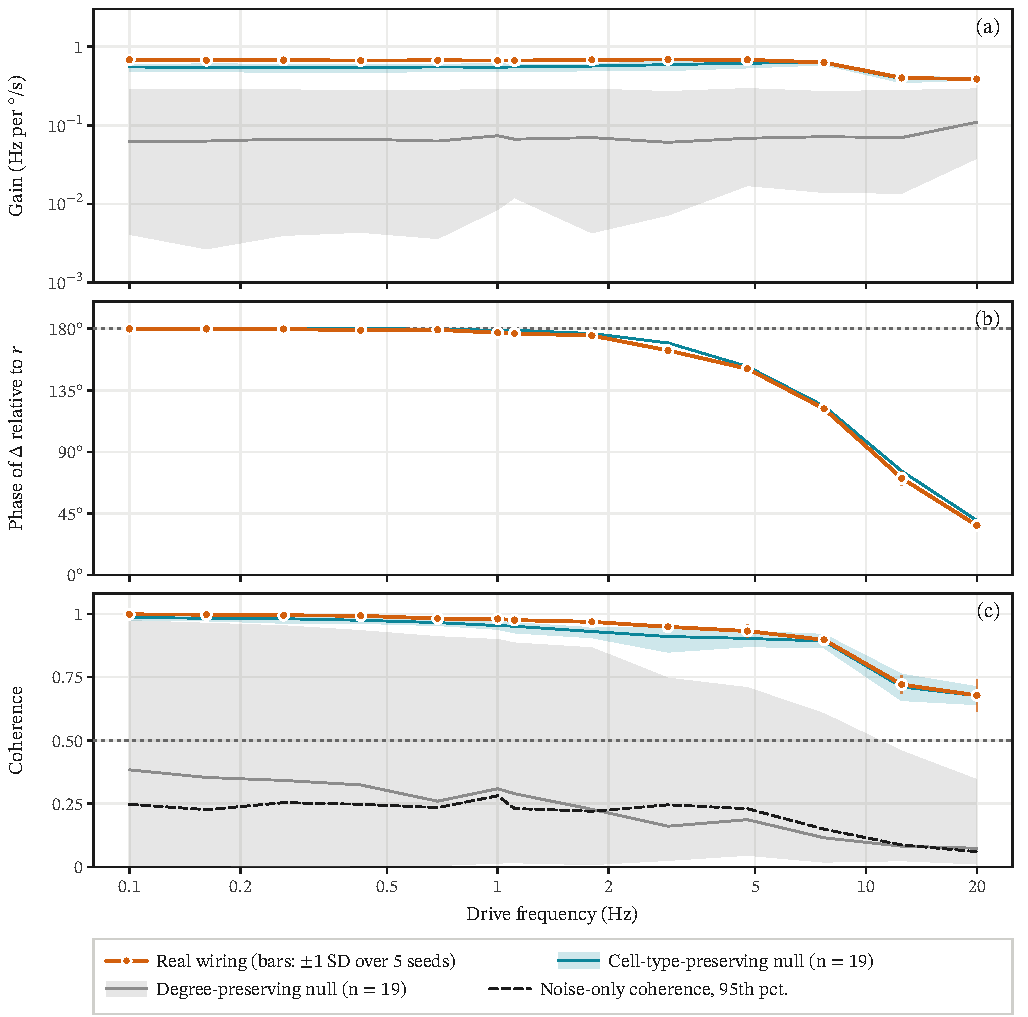
\includegraphics[width=1\linewidth,height=\textheight,keepaspectratio,alt={Bode plot of the real wiring against both null models}]{figures/fig1.pdf}
\caption{\textbf{Figure 1. Open-loop frequency response of the real
wiring and of both null models.} Right-minus-left DNa02 rate Δ in
response to yaw rate \emph{r} (100~°/s stepped sines, mean of 5 seeds).
(a) Gain, (b) phase of Δ relative to \emph{r} (180° opposes the
rotation), (c) coherence. Vertical bars on the real wiring: ±1 SD over
the 5 seeds. In (a) and (c), bands span the minimum to maximum of the 19
rewirings of each null and thin lines are their medians. Panel (b) shows
the cell-type-preserving median only (no band), because most
degree-preserving rewirings have too little coherence for a phase to be
defined; its dotted line marks 180°. The dotted line in (c) is the H1
threshold; the dashed line is the 95th percentile of the coherence of a
sine against white noise, computed for a single seed.}\label{f-bode}
\end{figure}

\protect\phantomsection\label{t-h1}
\begin{longtable}[]{@{}lrrrrr@{}}
\caption{\textbf{Table 2. Pre-specified H1 test at 1~Hz.} The real
wiring against 19 rewirings of each null. Rank 1 is the highest value;
\emph{p} from Eq.~(15).}\tabularnewline
\toprule\noalign{}
Measure & Real & Null median & Null max. & Rank & \emph{p} \\
\midrule\noalign{}
\endfirsthead
\toprule\noalign{}
Measure & Real & Null median & Null max. & Rank & \emph{p} \\
\midrule\noalign{}
\endhead
\bottomrule\noalign{}
\endlastfoot
\multicolumn{6}{@{}l@{}}{%
\emph{Degree-preserving null}} \\
 Coherence & 0.980 & 0.309 & 0.898 & 1 of 20 & 0.05 \\
 Gain (Hz per °/s) & 0.666 & 0.075 & 0.290 & 1 of 20 & 0.05 \\
\multicolumn{6}{@{}l@{}}{%
\emph{Cell-type-preserving null}} \\
 Coherence & 0.980 & 0.953 & 0.970 & 1 of 20 & 0.05 \\
 Gain (Hz per °/s) & 0.666 & 0.550 & 0.609 & 1 of 20 & 0.05 \\
\end{longtable}

\subsection{\texorpdfstring{3.2\quad Closed-loop gust rejection (H2, H2b
and
H3)}{3.2Closed-loop gust rejection (H2, H2b and H3)}}\label{closed-loop-gust-rejection-h2-h2b-and-h3}

\noindent The closed-loop tests asked whether the circuit, wired to the
rudder, reduces the aircraft's yaw response to gusts, and whether the
real wiring does so better than scrambled wirings given the same tuning.
The tuning rule selected \emph{K}~=~0.0139 per Hz for the real wiring
and \emph{K}~=~7.2 per rad/s for the yaw damper, on both models. At this
gain the fly loop's largest measured \textbar{}\emph{L}\textbar{} was
0.55 (at 0.34~Hz, phase +6°), so \textbar{}\emph{L}\textbar~\textless~1
at every tested frequency and no phase margin applies. Its nominal gain
margin is 34~dB at the 0.06~Hz phase crossing, where
\textbar{}\emph{L}\textbar~=~0.019 is near the measurement noise floor
(up to 0.012). Above about 3~Hz \textbar{}\emph{L}\textbar{} falls below
the noise floor at several grid points (3.6, 5.9, 33, 50~Hz) and the
phase there is unresolved, so a crossing in that range cannot be ruled
out. \textbar{}\emph{L}\textbar{} was at most 0.06 at every tested
frequency from 2~Hz up, so the gain margin would remain well above the
6~dB threshold even if the phase crossed −180° at any of those
frequencies. These are finite-amplitude, single-seed estimates on the
two-state model (Section 2.7). The damper had 31.9~dB and 61.3°. The fly
loop is admissible because its gain is low. No controller departed
controlled flight on any test seed.

The real wiring reduced RMS yaw rate on both models (Table~3, Fig.~2).
On the six-degree-of-freedom model the paired difference real~−~bare was
−0.73 {[}95\% CI −0.81, −0.64{]}~°/s, a 19\% reduction; on the two-state
model it was −0.45 {[}95\% CI −0.53, −0.36{]}~°/s (14\%). H2 and H3 were
supported. Real~−~median scrambled was −0.72 {[}95\% CI −0.80,
−0.64{]}~°/s and −0.44 {[}95\% CI −0.53, −0.36{]}~°/s. The interval
excludes 0 on both models, so H2b was supported as pre-specified; the
real wiring also had the lowest mean RMS yaw rate of all 11 wirings on
both models, although with 10 rewirings that rank cannot reach \emph{p}
below 1/11~≈~0.091. Three caveats temper this. First, H2b is a paired
difference conditional on these ten tuned rewirings, not an estimate
over all possible rewirings. Second, the tuning rule set \emph{K}~=~0
(no rudder command, so the controller flies as the bare airframe) for
five of 10 scrambled wirings on the two-state model and three on the
six-degree-of-freedom model, which pulls the median scrambled controller
toward the bare airframe. On the two-state model the median scrambled
wiring equals the bare airframe on 16 of 20 seeds, and H2b nearly
repeats H2 (−0.44 against −0.45~°/s), so the per-wiring ranking is the
more informative comparison. Finally, the scrambled wiring with the
lowest mean RMS yaw rate came within 4\% of the real wiring on the
six-degree-of-freedom model (scrambled 08) and 10\% on the two-state
model (scrambled 02); Section 3.3 shows how the closest ones achieved
this. When each scrambled wiring's readout sign was instead taken from
its own open-loop response, the real wiring still ranked first
(real~−~median −0.62 {{[}−0.69, −0.56{]}} and −0.42 {{[}−0.50,
−0.35{]}}~°/s).

The classical yaw damper was far better: 57\% and 52\% less RMS yaw rate
than the bare airframe, and damper~−~real of −1.51 {[}95\% CI −1.63,
−1.39{]} and −1.15 {[}95\% CI −1.27, −1.04{]}~°/s. On sideslip the
picture differs. The real wiring lowered RMS sideslip against the bare
airframe on both models (−0.25 {{[}−0.28, −0.21{]}}° and −0.08
{{[}−0.11, −0.05{]}}°), and on the two-state model its mean RMS sideslip
(1.63°) was below the yaw damper's (1.76°), whose difference from bare
there was 0.05 {{[}−0.03, 0.13{]}}°. An exploratory arm with a four-fold
stronger input gain (\emph{γ}~=~4, two-state model only) reached
2.08~°/s, a difference from bare of −1.01 {{[}−1.17, −0.87{]}}~°/s. The
real wiring is therefore a yaw damper that helps on every test seed, but
a much weaker one than the classical design.

\protect\phantomsection\label{t-cl}
\begin{longtable}[]{@{}lrrrr@{}}
\caption{\textbf{Table 3. Closed-loop performance in moderate
turbulence.} Mean RMS yaw rate and RMS sideslip on 20 held-out test
seeds, with 95\% bootstrap intervals over seeds. For the 10 scrambled
wirings the range of their means is given. Bare: no yaw controller; on
the six-degree-of-freedom model the wings-level roll hold common to
every controller stays on.}\tabularnewline
\toprule\noalign{}
& \multicolumn{2}{c}{%
Two-state model} & \multicolumn{2}{c@{}}{%
JSBSim 6-DOF} \\
Controller & RMS \emph{r} (°/s) & RMS \emph{β} (°) & RMS \emph{r} (°/s)
& RMS \emph{β} (°) \\
\midrule\noalign{}
\endfirsthead
\toprule\noalign{}
& \multicolumn{2}{c}{%
Two-state model} & \multicolumn{2}{c@{}}{%
JSBSim 6-DOF} \\
Controller & RMS \emph{r} (°/s) & RMS \emph{β} (°) & RMS \emph{r} (°/s)
& RMS \emph{β} (°) \\
\midrule\noalign{}
\endhead
\bottomrule\noalign{}
\endlastfoot
No yaw controller (bare) & 3.09 {{[}2.90, 3.29{]}} & 1.71 {{[}1.62,
1.81{]}} & 3.92 {{[}3.72, 4.12{]}} & 2.01 {{[}1.91, 2.12{]}} \\
Yaw damper & 1.50 {{[}1.42, 1.58{]}} & 1.76 {{[}1.68, 1.85{]}} & 1.69
{{[}1.59, 1.79{]}} & 1.73 {{[}1.64, 1.81{]}} \\
Fly, real wiring & 2.65 {{[}2.50, 2.81{]}} & 1.63 {{[}1.55, 1.72{]}} &
3.19 {{[}3.05, 3.33{]}} & 1.77 {{[}1.69, 1.85{]}} \\
Fly, scrambled wirings & 2.91--3.09 & 1.67--1.71 & 3.31--3.94 &
1.99--7.41 \\
Rank of real among wirings & 1 of 11 & 1 of 11 & 1 of 11 & 1 of 11 \\
\end{longtable}

\begin{figure}
\centering
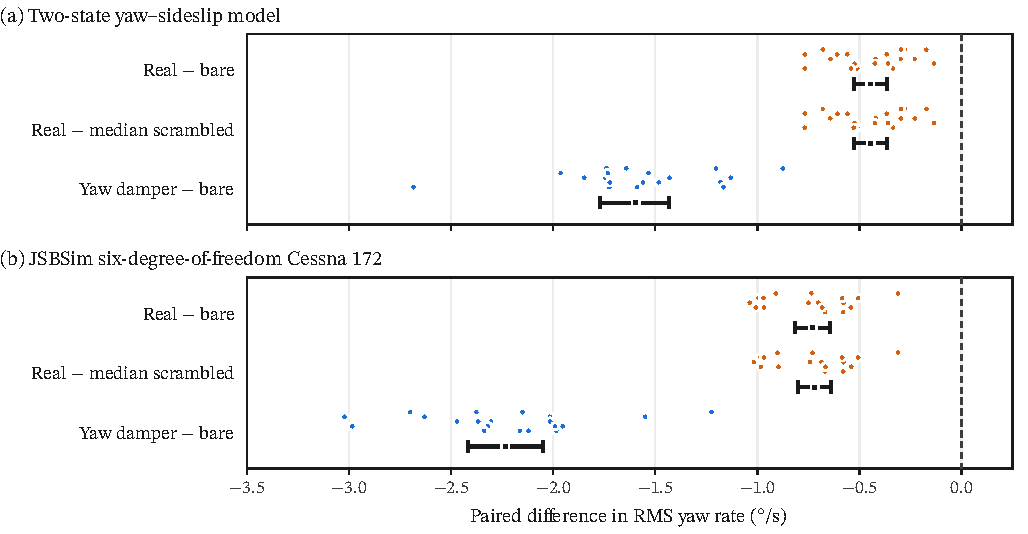
\includegraphics[width=1\linewidth,height=\textheight,keepaspectratio,alt={Per-seed paired differences in RMS yaw rate}]{figures/fig2.pdf}
\caption{\textbf{Figure 2. Paired differences in RMS yaw rate on the 20
held-out test seeds.} Small dots: one per seed. Squares and bars: mean
and 95\% percentile bootstrap interval. Negative values favour the
first-named controller. The real wiring helps on every seed; the yaw
damper helps much more.}\label{f-paired}
\end{figure}

\subsection{\texorpdfstring{3.3\quad Scrambled controllers that reduce
yaw rate by skidding (secondary
analysis)}{3.3Scrambled controllers that reduce yaw rate by skidding (secondary analysis)}}\label{scrambled-controllers-that-reduce-yaw-rate-by-skidding-secondary-analysis}

\noindent The scrambled wirings that came closest to the real wiring on
yaw rate were not better yaw dampers. The tuning rule chose each gain by
RMS yaw rate on the training gusts alone, and that statistic barely
penalizes a slow, steady turn, so a controller can score well by holding
the rudder over and letting the aircraft skid round. On the
six-degree-of-freedom model, scrambled wirings 01, 02 and 08 selected
\emph{K}~=~0.268 per Hz, a value reached only after the grid widening.
At this gain the command is saturated in 100\% of control steps for
each: the controller has become a relay that slams the rudder to one
stop or the other. In the replayed flights, the sparse DNa02 spike train
passed through the washout keeps the relay mostly on one side, holding a
steady rudder deflection, so the aircraft flies a slow, skidding turn.
RMS yaw rate, the pre-specified statistic, barely penalizes a slow
steady turn; RMS sideslip does. Across all test seeds only RMS sideslip
was checked: averaged over the seeds, these three controllers had RMS
sideslip of 7.1--7.4°, against 2.01° for the bare airframe, 1.73° for
the yaw damper and 1.77° for the real wiring (Fig.~3). By RMS sideslip,
a measure recorded under the protocol but not used as a test statistic,
the real wiring ranks first of 11 on both models.

The replay of test seed 100 shows the mechanism directly (Fig.~4,
Table~4; it is also the scenario replayed in the viewer above).
Scrambled wiring 08 held a mean rudder of +11.5° with the rudder
saturated in 100\% of steps, turned the heading by +64° (to the right)
in 60~s at a mean sideslip of −7.2°, and ended 1.72~km right of the bare
airframe's path. The real wiring and the yaw damper stayed within 21~m
of it. The scrambled controller with the lowest RMS yaw rate is
therefore not a usable yaw damper, and the near-tie on RMS yaw rate in
Section 3.2 is an artefact of that metric.

\begin{figure}
\centering
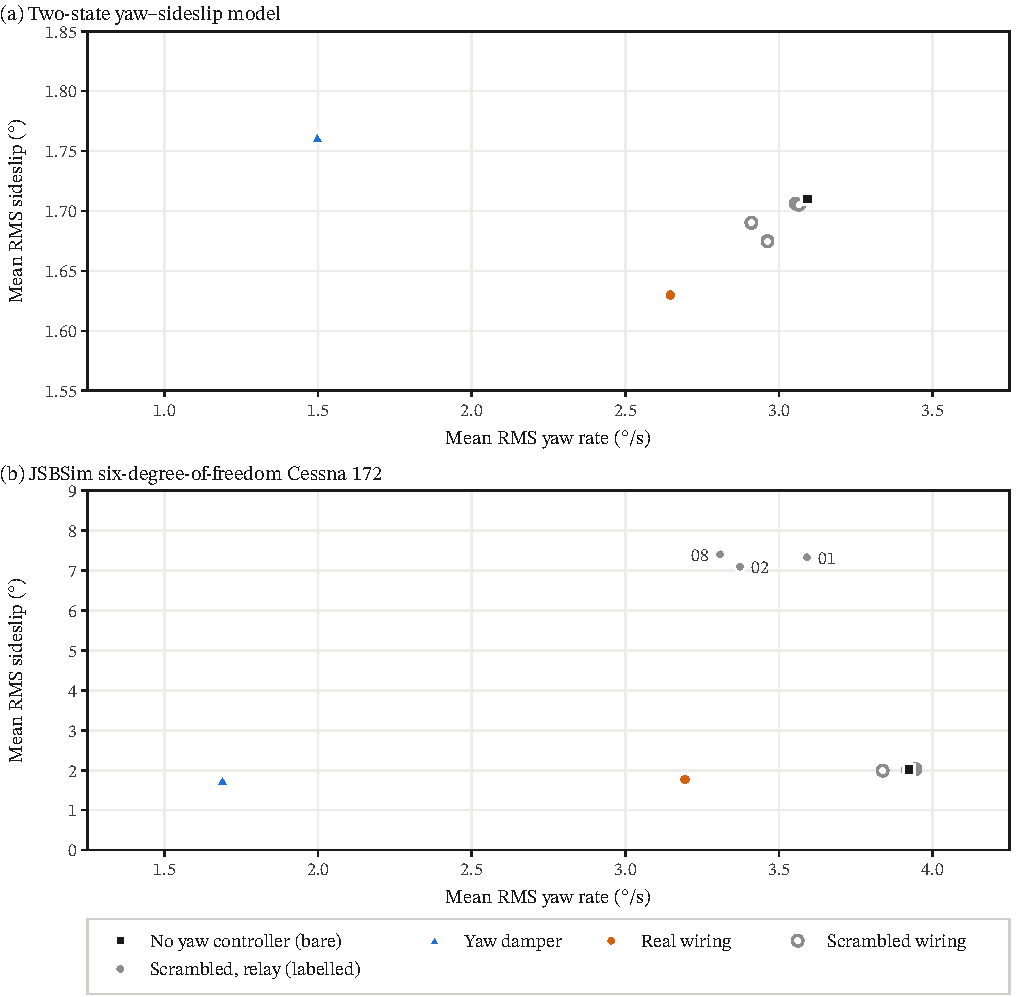
\includegraphics[width=1\linewidth,height=\textheight,keepaspectratio,alt={RMS sideslip against RMS yaw rate for every controller}]{figures/fig3.pdf}
\caption{\textbf{Figure 3. RMS sideslip against RMS yaw rate for every
controller.} Means over the 20 test seeds. A good yaw damper sits low on
both axes. Filled grey points are scrambled wirings whose rudder was
saturated in more than 90\% of steps (relays); several scrambled wirings
with \emph{K}~=~0 coincide with the bare airframe. Note the different
sideslip scales: the axis in (a) is expanded, while (b) must also hold
the relays. Bare: no yaw controller; on the six-degree-of-freedom model
the wings-level roll hold common to every controller stays
on.}\label{f-scatter}
\end{figure}

\begin{figure}
\centering
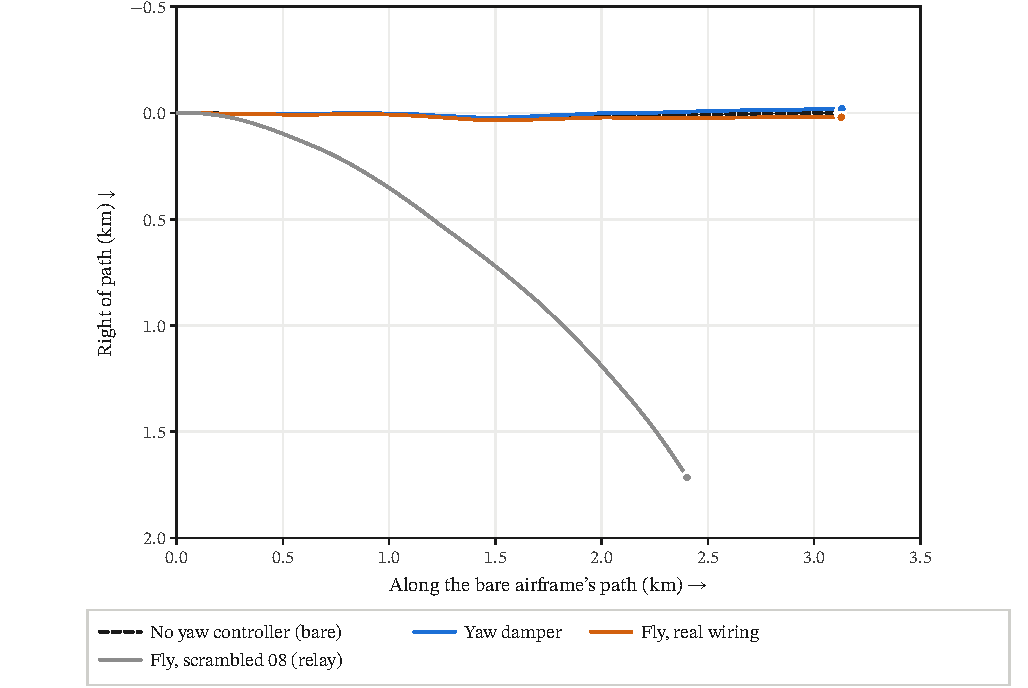
\includegraphics[width=1\linewidth,height=\textheight,keepaspectratio,alt={Ground tracks of the seed-100 flights, plan view from above}]{figures/fig4.pdf}
\caption{\textbf{Figure 4. Ground tracks of the six-degree-of-freedom
flights on test seed 100.} Same turbulence random seed for all. JSBSim's
gust filter depends on each aircraft's airspeed, so the gust histories
differ slightly: at most about 0.06~m/s for the controllers shown,
0.47~m/s for the skidding relay. Plan view from above. Scrambled wiring
08 had the lowest training RMS yaw rate of the ten scrambled wirings,
but it flies as a relay: the rudder sits at its stop, the aircraft skids
in a steady right turn and ends 1.72~km off course (Section 3.3). The
frame is aligned with the bare airframe's start-to-end path, which runs
left to right, so a turn to the right appears as a track bending
downward; both axes have the same scale. Dots mark the end of each 60~s
flight. Bare: no yaw controller; on the six-degree-of-freedom model the
wings-level roll hold common to every controller stays
on.}\label{f-tracks}
\end{figure}

\protect\phantomsection\label{t-replay}
\begin{longtable}[]{@{}lrrrrr@{}}
\caption{\textbf{Table 4. Rudder use and flight path on test seed 100.}
Computed from the replayed flights: mean rudder deflection (commanded
deflection relative to trim), fraction of steps with the rudder at its
stop, heading change over the flight (+ = right), final offset to the
right (+) of the bare airframe's path, and mean sideslip. Bare: no yaw
controller; on the six-degree-of-freedom model the wings-level roll hold
common to every controller stays on.}\tabularnewline
\toprule\noalign{}
Flight & Mean rudder (°) & Saturated & Heading (°) & Offset (m) & Mean
\emph{β} (°) \\
\midrule\noalign{}
\endfirsthead
\toprule\noalign{}
Flight & Mean rudder (°) & Saturated & Heading (°) & Offset (m) & Mean
\emph{β} (°) \\
\midrule\noalign{}
\endhead
\bottomrule\noalign{}
\endlastfoot
\multicolumn{6}{@{}l@{}}{%
\emph{Six-degree-of-freedom model}} \\
 No yaw controller (bare) & 0.00 & 0\% & −5.2 & 0 & 0.05 \\
 Yaw damper & 0.00 & 0\% & −5.1 & −20 & 0.02 \\
 Real wiring & +0.14 & 3\% & −4.1 & +21 & −0.05 \\
 Scrambled 08 & +11.47 & 100\% & +63.8 & +1715 & −7.20 \\
 Scrambled 00 & +0.08 & 1\% & −4.7 & +12 & 0.00 \\
\multicolumn{6}{@{}l@{}}{%
\emph{Two-state model}} \\
 No yaw controller (bare) & 0.00 & 0\% & −1.7 & 0 & −0.04 \\
 Yaw damper & −0.01 & 0\% & −2.7 & 0 & 0.00 \\
 Real wiring & +0.12 & 2\% & −1.4 & +10 & −0.11 \\
 Scrambled 02 & +0.39 & 15\% & +0.3 & +34 & −0.29 \\
 Scrambled 00 & 0.00 & 0\% & −1.7 & 0 & −0.03 \\
\end{longtable}

\subsection{\texorpdfstring{3.4\quad Neuron loss
(H4)}{3.4Neuron loss (H4)}}\label{neuron-loss-h4}

\noindent The lesion experiment asked how the controller degrades as its
neurons are silenced, and whether the real wiring degrades more
gracefully than scrambled wirings. No flight departed controlled flight:
0 of the 1,040 flights of the lesion experiment (960 with neurons
silenced), across 4 wirings, every lesion condition and 20 test seeds.
Every AUC in Eq.~(16) is therefore 1, and the difference is 0, with a
degenerate bootstrap interval (no departures). The bare Cessna with its
wings-level hold does not depart in moderate turbulence, so H4 could not
be tested as pre-specified; the Wilson 95\% upper bound on the departure
probability in each cell is 0.16.

The pre-specified secondary measure, mean RMS yaw rate, was informative
(Fig.~5). As neurons were silenced at random, the real wiring's mean RMS
yaw rate rose from 3.19~°/s to the bare airframe's 3.92~°/s, losing 38\%
of its benefit at 5\% and reaching the bare value (to two decimals) by
60\%; the increase by 80\% was 0.73 {{[}0.64, 0.81{]}}~°/s. Its worst
mean in any lesion condition was 3.92~°/s, so its mean RMS yaw rate
stayed at or below the bare value in every condition. One of 240
lesioned flights was slightly worse than bare on the same seed (seed 108
at 5\%: 3.387 against 3.372~°/s). Its difference from the mean of the
scrambled wirings stayed below zero up to 60\% silenced (95\% intervals)
and approached zero beyond, as all controllers converged on the bare
airframe. Two of the three scrambled wirings in this experiment (01 and
02) are the relay controllers of Section 3.3, and they behaved
differently: under some lesions their mean RMS yaw rate was above the
bare airframe's, up to 5.07 and 5.49~°/s. The neuron-loss replay in the
viewer above shows the real wiring at 0\%, 40\% and 80\% random loss and
with its HS cells silenced.

Part of this fade is loss of the readout itself. In the intact replays
of test seed 100 the right DNa02 fired no spikes on either aircraft
model, while the left fired 153 in 60~s (2.55~Hz), so the rudder command
came from the left DNa02 alone. Silencing the left DNa02 therefore
switches the controller off unless the lesion lets the right one fire.
At 5\% the left DNa02 was silenced on 6 of 20 seeds (about 1 expected);
five of these flights were identical to the bare airframe, and on the
other (seed 103) the controller still steered, so the right DNa02 must
have fired. These five switched-off seeds account for 55\% of the 38\%
of benefit lost at 5\%; the other 15 seeds lost 21\%. The number of
flights identical to the bare airframe rose with the lesion fraction: 5,
5, 9, 15, 18 and 20 of 20 at 5\%, 10\%, 20\%, 40\%, 60\% and 80\%. At
the higher fractions some of them (1 at 20\%, 3 at 40\%, 3 at 60\%, 2 at
80\%) kept an intact left DNa02 and were switched off by loss upstream.
The lesion curve therefore mixes loss of processing with loss of the
single active readout cell.

Targeted lesions locate the function (Table~5). Silencing the six HS
cells returned the real wiring exactly to the bare airframe's RMS yaw
rate; HS cells were necessary for its closed-loop effect in this model.
Silencing all T4 or all T5 cells left part of the function (3.59 and
3.75~°/s), and in both cases the real wiring stayed below the scrambled
mean (−1.03 {{[}−1.13, −0.93{]}} and −0.72 {{[}−0.81, −0.63{]}}~°/s).
With HS silenced the real wiring was worse than the scrambled mean
(+0.30 {{[}0.20, 0.39{]}}~°/s), because the relay wirings do not depend
on HS. The hub lesions are uninformative by construction: the
top-betweenness sets of the real wiring contain both DNa02 readout
neurons and all 6 HS cells, so silencing them removes the readout
itself, and every wiring then flew exactly like the bare airframe. Under
random neuron loss, then, the real wiring's mean degrades toward the
bare airframe but not beyond it, and HS cells were necessary for its
effect.

\begin{figure}
\centering
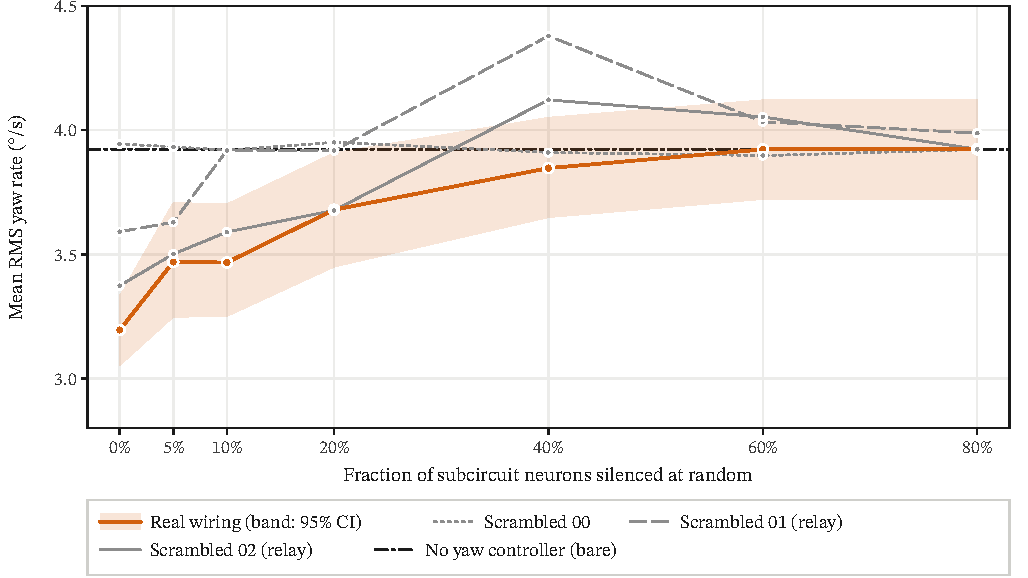
\includegraphics[width=1\linewidth,height=\textheight,keepaspectratio,alt={RMS yaw rate against random lesion fraction}]{figures/fig5.pdf}
\caption{\textbf{Figure 5. Mean RMS yaw rate against the fraction of
neurons silenced at random.} Mean over 20 test seeds (nested sets, the
same neurons in every wiring), on the six-degree-of-freedom model. Each
wiring keeps its tuned gain. The shaded band is the 95\% bootstrap
interval for the real wiring; the dash-dotted line is the bare airframe.
The yaw damper, for reference, flies at 1.69~°/s. Bare: no yaw
controller; on the six-degree-of-freedom model the wings-level roll hold
common to every controller stays on.}\label{f-lesion}
\end{figure}

\protect\phantomsection\label{t-targeted}
\begin{longtable}[]{@{}lrrrrr@{}}
\caption{\textbf{Table 5. Targeted lesions.} Mean RMS yaw rate (°/s)
over 20 test seeds on the six-degree-of-freedom model, and the paired
difference between the real wiring and the mean of the scrambled wirings
with its 95\% bootstrap interval. The bare airframe flies at 3.92~°/s;
no flight departed.}\tabularnewline
\toprule\noalign{}
Silenced & Real & Scr. 00 & Scr. 01 & Scr. 02 & Real − scr. mean \\
\midrule\noalign{}
\endfirsthead
\toprule\noalign{}
Silenced & Real & Scr. 00 & Scr. 01 & Scr. 02 & Real − scr. mean \\
\midrule\noalign{}
\endhead
\bottomrule\noalign{}
\endlastfoot
None & 3.19 & 3.94 & 3.59 & 3.37 & −0.44 {{[}−0.51, −0.37{]}} \\
All HS cells & 3.92 & 3.93 & 3.57 & 3.39 & +0.30 {{[}0.20, 0.39{]}} \\
All T4 cells & 3.59 & 3.92 & 5.07 & 4.88 & −1.03 {{[}−1.13, −0.93{]}} \\
All T5 cells & 3.75 & 3.92 & 3.98 & 5.49 & −0.72 {{[}−0.81, −0.63{]}} \\
Hubs, top 5\% & 3.92 & 3.92 & 3.92 & 3.92 & 0.000 {{[}0.000,
0.000{]}} \\
Hubs, top 10\% & 3.92 & 3.92 & 3.92 & 3.92 & 0.000 {{[}0.000,
0.000{]}} \\
Hubs, top 20\% & 3.92 & 3.92 & 3.92 & 3.92 & 0.000 {{[}0.000,
0.000{]}} \\
\end{longtable}

\subsection{\texorpdfstring{3.5\quad Amplitude dependence and full-brain
check (exploratory and planned
checks)}{3.5Amplitude dependence and full-brain check (exploratory and planned checks)}}\label{amplitude-dependence-and-full-brain-check-exploratory-and-planned-checks}

\noindent Two further analyses asked whether the open-loop results,
measured at large amplitude in an isolated subcircuit, carry over to the
conditions of the closed-loop flights. The open-loop measurements used
100~°/s, but in turbulence the bare airframe yaws at about 3--4~°/s RMS
(3.1 on the two-state, 3.9 on the six-degree-of-freedom model). In an
exploratory sweep at 1~Hz, coherence fell from 0.98 at 100~°/s to 0.67
at 3~°/s, while the lock-in gain rose to 1.2--1.4~Hz per °/s, partly a
noise bias at low coherence and partly nonlinearity. The real wiring
still had the highest coherence of the 20 wirings (real and
degree-preserving) at every amplitude. At rest, DNa02 fired at 1.4~Hz on
the left and 0.0~Hz on the right, so at turbulence-level yaw rates a
single readout neuron per side operates near threshold and the signal
reaching the rudder is sparse and partly rectified. This is consistent
with the low loop gain of Section 3.2 and with the improvement seen at a
stronger input gain. In a planned sensitivity check across input gains
\emph{γ} from 0.5 to 4, coherence up to 2~Hz stayed above 0.83.

In a planned check of what the subcircuit leaves out, the real wiring
was also run inside the whole v783 brain (all connections, with no
5-synapse cutoff, and all 12,246 T4/T5 cells as sources, against 12,056
in the subcircuit) at 0.5, 2.0 and 8.0~Hz (2 seeds). The subcircuit kept
the full brain's phase to within 3.9°, but its gain was 15--17\% lower
at 0.5--2~Hz and 36\% lower at 8~Hz. The large-amplitude
characterization therefore describes the circuit under strong drive: at
turbulence-level yaw rates its output is weaker and noisier. The
subcircuit's lower gain combines the restored weak connections, the
extra neurons and the extra sources of the whole brain, and is not
attributable to isolation alone.

\protect\phantomsection\label{s4}
\section{\texorpdfstring{4\quad Discussion}{4Discussion}}\label{discussion}

\subsection{\texorpdfstring{4.1\quad Principal
findings}{4.1Principal findings}}\label{principal-findings}

\noindent Treated as a flight-control element and driven at large
amplitude (100~°/s), this model of the fly's visual yaw pathway behaves
like a delayed rate sensor; at the few-degrees-per-second yaw rates of
turbulence its output becomes noisy and partly rectified (Section 3.5).
It tracks yaw rotation coherently from 0.1 to several hertz, with the
sign a stabilizing reflex needs and an effective high-frequency
phase-slope delay of about 22~ms. That property depends on the wiring:
rewiring that keeps every neuron's degree and sign but scrambles which
cell types connect on which side removes most of the response. Most of
it survives a rewiring that respects cell type and side, but that
rewiring leaves the core T4/T5~→~HS~→~DNa02 connections intact, so it
shows only that the remaining connections contribute a small, consistent
increment.

Closed around a rudder, the circuit is a weak but real yaw damper. It
improves on the bare airframe on every test seed, and it ranks first
among the wirings on yaw rate and on sideslip, but the classical yaw
damper, tuned by the same rule with the same budget, removes about three
times (six-degree-of-freedom) to three and a half times (two-state) as
much yaw motion. Under random neuron loss the real wiring's mean RMS yaw
rate stayed at or below the bare airframe's in every condition (one of
240 lesioned flights was slightly worse), partly because losing its
single active readout neuron switches it off; relay-type scrambled
controllers had mean RMS yaw rate above the bare airframe's under some
lesions.

\subsection{\texorpdfstring{4.2\quad What limits the fly
controller}{4.2What limits the fly controller}}\label{what-limits-the-fly-controller}

\noindent Latency is unlikely to be the main limit: at 100~°/s the
circuit's phase lag near the Dutch-roll frequency is at most 1.2°, and
its measured \textbar{}\emph{L}\textbar{} never exceeded 0.55 (Section
3.2). The evidence points instead to signal strength: in turbulence the
T4/T5 input is small, the single DNa02 neuron on each side fires near
threshold (in the intact replays only the left one fired), and the
RMS-optimal gain (which the margin rule did not bind) is low because
higher gain adds more spike noise to the rudder than it removes yaw
motion; the exploratory stronger-input arm is consistent with this.

\subsection{\texorpdfstring{4.3\quad Comparison with prior work and with
flies}{4.3Comparison with prior work and with flies}}\label{comparison-with-prior-work-and-with-flies}

\noindent The model's effective phase-slope delay is of the same order
as the delays of tens of milliseconds measured for the optomotor
response in tethered flight \cite{theobald2010}; this comparison is
qualitative only. Behavioural yaw linear filters exist
\cite{theobald2010} but differ in stimulus, output (wingbeat amplitude)
and processing stages, and descending-neuron impulse responses used roll
stimuli \cite{leibbrandt2021}, so we compare only delays. Earlier
connectome flight-loop projects reported time-domain behaviour,
sometimes against shuffled wiring
\cite{clutch2026,leohio2026,flygm2026}. The frequency-response, margin,
turbulence and lesion measurements reported here complement such
demonstrations, and they use the same kind of shuffled-wiring control.

\subsection{\texorpdfstring{4.4\quad Evaluating connectome
controllers}{4.4Evaluating connectome controllers}}\label{evaluating-connectome-controllers}

\noindent The relay controllers carry a methodological lesson. Our
primary metric, RMS yaw rate, together with a pre-specified rule to
widen the gain grid, admitted controllers that reduce yaw rate by
holding the rudder over and skidding in a steady turn. The margin
constraint did not exclude them: measured by injection on the two-state
model, where a saturated loop yields only a describing-function margin,
they showed gain margins of 7.5--12.1~dB. Similarly, the departure-based
lesion test could not discriminate between wirings because nothing
departed. In both cases the pre-specified statistic was blind to a
difference that a second measure, sideslip or mean RMS yaw rate,
revealed.

\subsection{\texorpdfstring{4.5\quad Limitations}{4.5Limitations}}\label{limitations}

\noindent The conclusions are about this model of the wiring, not about
real flies. The whole-brain model was validated on gustatory and
grooming circuits, not on visual neurons \cite{shiu2024}, and on
connectome release v630; we run it on v783. The model omits gap
junctions, which carry much of the coupling between HS and H2 cells, and
it treats graded-potential neurons such as T4/T5, HS and VS cells as
spiking ones \cite{shiu2024,pokusaeva2024}. Our input encoding is
piecewise linear (half-wave rectified) in \emph{r} for each cell and
ignores the temporal-frequency tuning and pattern dependence of motion
detectors. DNa02's steering role is established in walking
\cite{rayshubskiy2025}, and its role in flight is inferred from
connectivity. The subcircuit underestimates the full brain's gain, by up
to 36\% at 8~Hz. Loop margins were measured on the two-state model only
and reused for the six-degree-of-freedom model, whose turbulence model
differs in spectral shape. With 10 scrambled wirings in closed loop the
smallest attainable \emph{p} is 0.091, so the closed-loop ranking is
suggestive rather than significant at 0.05 on its own. All flights used
one aircraft loading (2,480 lb, centre of gravity 45.5 in aft of the
datum and 4.2 in right of the centreline, from the default seat masses);
a longitudinal shift of the centre of gravity changes the fin's moment
arm and hence the yaw damping, and a lateral offset mainly changes trim;
neither was varied. The margin thresholds were applied as a screening
rule, not as a full MIL-F-9490D compliance test (Section 2.7).

\subsection{\texorpdfstring{4.6\quad Future
work}{4.6Future work}}\label{future-work}

\noindent A future protocol should constrain mean rudder, sideslip or
heading drift, and measure margins on the plant being flown. A
discriminating lesion test would need a harsher plant or turbulence
level, and hub sets that exclude the readout neurons. More closed-loop
rewirings would let the per-wiring ranking reach conventional
significance, and a null that rewires the core T4/T5~→~HS~→~DNa02
connections neuron by neuron would test whether their neuron-level
wiring matters. Both controllers studied here are inner-loop yaw dampers
whose washout passes steady turns, so neither tries to hold heading or
track. The natural next study places each inside conventional heading
and track loops, measures path error and recovery from discrete
disturbances, and tests whether other connectome pathways, such as the
VS cells that respond to roll and pitch, can drive the ailerons and
elevator, each compared with a conventional controller tuned by the same
rule.

\protect\phantomsection\label{s5}
\section{\texorpdfstring{5\quad Conclusions}{5Conclusions}}\label{conclusions}

\noindent A spiking model of the fruit fly's visual yaw pathway, taken
directly from the connectome and tested with the methods used to assess
a flight-control law, behaved as a delayed yaw-rate sensor with the
stabilizing sign and, closed around a rudder, as a weak yaw damper that
ranked first among the wirings tested, although with too few rewirings
for that rank alone to be significant. Its function depended on its
wiring and, in this model, required the HS cells, and under random
neuron loss its mean RMS yaw rate rose toward the bare airframe's value
without exceeding it, in part because the loss often silenced its one
active readout neuron. The same tests exposed scrambled controllers that
scored well on the primary metric by skidding, which argues for judging
connectome controllers, like any flight-control law, on several measures
and on the airframe they fly.

\protect\phantomsection\label{decl}
\section{Declarations}\label{declarations}

\subsection{Data and code
availability}\label{data-and-code-availability}

\noindent Code, result files and the replays shown in the viewer are
available at
\href{https://github.com/aryawidjaja/flight-test-the-fly}{\nolinkurl{github.com/aryawidjaja/flight-test-the-fly}},
archived on Zenodo as release v1.0.0
(doi:\href{https://doi.org/10.5281/zenodo.23156035}{\nolinkurl{10.5281/zenodo.23156035}}).
Closed-loop simulations ran at commit \texttt{393e70e}, open-loop at
\texttt{e5f90c0}, gain tuning at \texttt{bab4588} and \texttt{d98adb0}
and lesions at \texttt{ab35844} (47, 510, 432 and 104 result files).
These commits are archived privately, not on a public branch; the
analysis scripts were re-run on the public code from the stored per-job
results, and the simulations themselves were not re-run. The FlyWire
connectome and its annotations are available from their original
publications \cite{dorkenwald2024,schlegel2024}.

\subsection{Acknowledgements and
licences}\label{acknowledgements-and-licences}

\noindent Wiring data: the FlyWire Consortium, connectome v783,
CC~BY~4.0 \cite{dorkenwald2024,schlegel2024}. Neuron model and
connectivity table: Shiu et al., MIT licence \cite{shiu2024}. Flight
dynamics: JSBSim \cite{jsbsim2026}.

\subsection{AI assistance}\label{ai-assistance}

\noindent Generative AI: Claude Opus 5.5 (Anthropic), used through
Claude Code, assisted with writing and reviewing the simulation and
analysis code, running and checking the analyses, checking the
literature and citations, building the web viewer, and drafting and
editing the text. The author designed the study, made the methodological
decisions, checked the results and the text, and takes full
responsibility for the content.

\subsection{Competing interests}\label{competing-interests}

\noindent The author declares no competing interests.

\begin{thebibliography}{22}

\bibitem{dorkenwald2024}

\protect\phantomsection\label{ref-1}{Dorkenwald S, et al. (2024).
Neuronal wiring diagram of an adult brain. \emph{Nature} 634:124--138.
\href{https://doi.org/10.1038/s41586-024-07558-y}{\nolinkurl{doi:10.1038/s41586-024-07558-y}}}

\bibitem{schlegel2024}

\protect\phantomsection\label{ref-2}{Schlegel P, et al. (2024).
Whole-brain annotation and multi-connectome cell typing of
\emph{Drosophila}. \emph{Nature} 634:139--152.
\href{https://doi.org/10.1038/s41586-024-07686-5}{\nolinkurl{doi:10.1038/s41586-024-07686-5}}}

\bibitem{shiu2024}

\protect\phantomsection\label{ref-3}{Shiu PK, et al. (2024). A
\emph{Drosophila} computational brain model reveals sensorimotor
processing. \emph{Nature} 634:210--219.
\href{https://doi.org/10.1038/s41586-024-07763-9}{\nolinkurl{doi:10.1038/s41586-024-07763-9}}}

\bibitem{milf94901975}

\protect\phantomsection\label{ref-4}{US Air Force (6 June 1975).
MIL-F-9490D, \emph{Flight Control Systems -- Design, Installation and
Test of Piloted Aircraft, General Specification for}, §3.1.3.6.1, Table
III.}

\bibitem{milf87851980}

\protect\phantomsection\label{ref-5}{US Department of Defense (5
November 1980). MIL-F-8785C, \emph{Military Specification: Flying
Qualities of Piloted Airplanes}.
\href{https://everyspec.com/MIL-SPECS/MIL-SPECS-MIL-F/MIL-F-8785C_5295/}{\nolinkurl{everyspec.com/MIL-SPECS/MIL-SPECS-MIL-F/MIL-F-8785C_5295}}}

\bibitem{maisak2013}

\protect\phantomsection\label{ref-6}{Maisak MS, et al. (2013). A
directional tuning map of \emph{Drosophila} elementary motion detectors.
\emph{Nature} 500:212--216.
\href{https://doi.org/10.1038/nature12320}{\nolinkurl{doi:10.1038/nature12320}}}

\bibitem{shinomiya2019}

\protect\phantomsection\label{ref-7}{Shinomiya K, et al. (2019).
Comparisons between the ON- and OFF-edge motion pathways in the
\emph{Drosophila} brain. \emph{eLife} 8:e40025.
\href{https://pmc.ncbi.nlm.nih.gov/articles/PMC6338461/}{PMC6338461}}

\bibitem{schnell2010}

\protect\phantomsection\label{ref-8}{Schnell B, et al. (2010).
Processing of horizontal optic flow in three visual interneurons of the
\emph{Drosophila} brain. \emph{J Neurophysiol} 103:1646--1657.
\href{https://doi.org/10.1152/jn.00950.2009}{\nolinkurl{doi:10.1152/jn.00950.2009}}}

\bibitem{haikala2013}

\protect\phantomsection\label{ref-9}{Haikala V, et al. (2013).
Optogenetic control of fly optomotor responses. \emph{J Neurosci}
33:13927--13934.
\href{https://pmc.ncbi.nlm.nih.gov/articles/PMC6618655/}{PMC6618655}}

\bibitem{namiki2018}

\protect\phantomsection\label{ref-10}{Namiki S, et al. (2018). The
functional organization of descending sensory-motor pathways in
\emph{Drosophila}. \emph{eLife} 7:e34272.
\href{https://pmc.ncbi.nlm.nih.gov/articles/PMC6019073/}{PMC6019073}}

\bibitem{rayshubskiy2025}

\protect\phantomsection\label{ref-11}{Rayshubskiy A, et al. (2025).
Neural circuit mechanisms for steering control in walking
\emph{Drosophila}. \emph{eLife} 13:RP102230.
\href{https://doi.org/10.7554/eLife.102230}{\nolinkurl{doi:10.7554/eLife.102230}}}

\bibitem{theobald2010}

\protect\phantomsection\label{ref-12}{Theobald JC, Ringach DL, Frye MA
(2010). Dynamics of optomotor responses in \emph{Drosophila} to
perturbations in optic flow. \emph{J Exp Biol} 213:1366--1375.
\href{https://pmc.ncbi.nlm.nih.gov/articles/PMC2846167/}{PMC2846167}}

\bibitem{clutch2026}

\protect\phantomsection\label{ref-13}{ClutchMedia775 (2026).
fly-brain-drone. Software repository, commit d017a6c, accessed 3 Oct
2026.
\href{https://github.com/ClutchMedia775/fly-brain-drone}{\nolinkurl{github.com/ClutchMedia775/fly-brain-drone}}}

\bibitem{leohio2026}

\protect\phantomsection\label{ref-14}{leohio (2026).
connectome-fly-closedloop. Software repository, commit 56eae22.
\href{https://github.com/leohio/connectome-fly-closedloop}{\nolinkurl{github.com/leohio/connectome-fly-closedloop}}}

\bibitem{flygm2026}

\protect\phantomsection\label{ref-15}{Jin Z, Zhu Y, Zhang C, Sui Y
(2026). Whole-brain connectomic graph model enables whole-body
locomotion control in fruit fly (FlyGM). arXiv:2602.17997v3 (14 Jun
2026).
\href{https://arxiv.org/abs/2602.17997v3}{\nolinkurl{arxiv.org/abs/2602.17997v3}}}

\bibitem{leibbrandt2021}

\protect\phantomsection\label{ref-16}{Leibbrandt R, Nicholas S,
Nordström K (2021). The impulse response of optic flow-sensitive
descending neurons to roll m-sequences. \emph{J Exp Biol} 224:jeb242833.
\href{https://doi.org/10.1242/jeb.242833}{\nolinkurl{doi:10.1242/jeb.242833}}}

\bibitem{jsbsim2026}

\protect\phantomsection\label{ref-17}{Berndt JS, Coconnier B, De Marco
A, McLeod S (2026). JSBSim -- An Open Source Flight Dynamics Software
Library, v1.3.1. Software.
\href{https://doi.org/10.5281/zenodo.20258622}{\nolinkurl{doi:10.5281/zenodo.20258622}};
\href{https://github.com/JSBSim-Team/jsbsim}{\nolinkurl{github.com/JSBSim-Team/jsbsim}}}

\bibitem{yeager1998}

\protect\phantomsection\label{ref-18}{Yeager JC (1998). Implementation
and testing of turbulence models for the F18-HARV simulation.
NASA/CR-1998-206937.
\href{https://ntrs.nasa.gov/citations/19980028448}{\nolinkurl{ntrs.nasa.gov/citations/19980028448}}}

\bibitem{boeing94901975}

\protect\phantomsection\label{ref-19}{Boeing Co. (1975).
\emph{Background Information and User's Guide for MIL-F-9490D}.
AFFDL-TR-74-116 (NTIS AD-A029 074); reproduces the stability-margin
table of the specification.
\href{https://www.acgsc.org/history/Early\%20Fly-By-Wire\%20Redundancy\%20Studies/User\%27s\%20Guide\%20to\%20MIL-F-9490D.pdf}{acgsc.org}}

\bibitem{mansur2009}

\protect\phantomsection\label{ref-20}{Mansur MH, Lusardi JA, Tischler
MB, Berger T (2009). Achieving the best compromise between stability
margins and disturbance rejection performance. \emph{American Helicopter
Society 65th Annual Forum}, Grapevine, TX.
\href{https://www.sjsu.edu/researchfoundation/docs/AHS_2009_Mansur.pdf}{\nolinkurl{sjsu.edu/researchfoundation/docs/AHS_2009_Mansur.pdf}}}

\bibitem{phipson2010}

\protect\phantomsection\label{ref-21}{Phipson B, Smyth GK (2010).
Permutation P-values should never be zero: calculating exact P-values
when permutations are randomly drawn. \emph{Stat Appl Genet Mol Biol}
9(1):Article 39.
\href{https://doi.org/10.2202/1544-6115.1585}{\nolinkurl{doi:10.2202/1544-6115.1585}}}

\bibitem{pokusaeva2024}

\protect\phantomsection\label{ref-22}{Pokusaeva VO, Satapathy R,
Symonova O, Joesch M (2024). Bilateral interactions of optic-flow
sensitive neurons coordinate course control in flies. \emph{Nat Commun}
15:8830.
\href{https://doi.org/10.1038/s41467-024-53173-w}{\nolinkurl{doi:10.1038/s41467-024-53173-w}}}

\end{thebibliography}

\end{document}
